\subsection{Gesamtkonzept}
\todo[inline]{Printherstellung Sektion erstellen}
\label{chap:grundkonzept}
\begin{figure}[h]
	\centering
	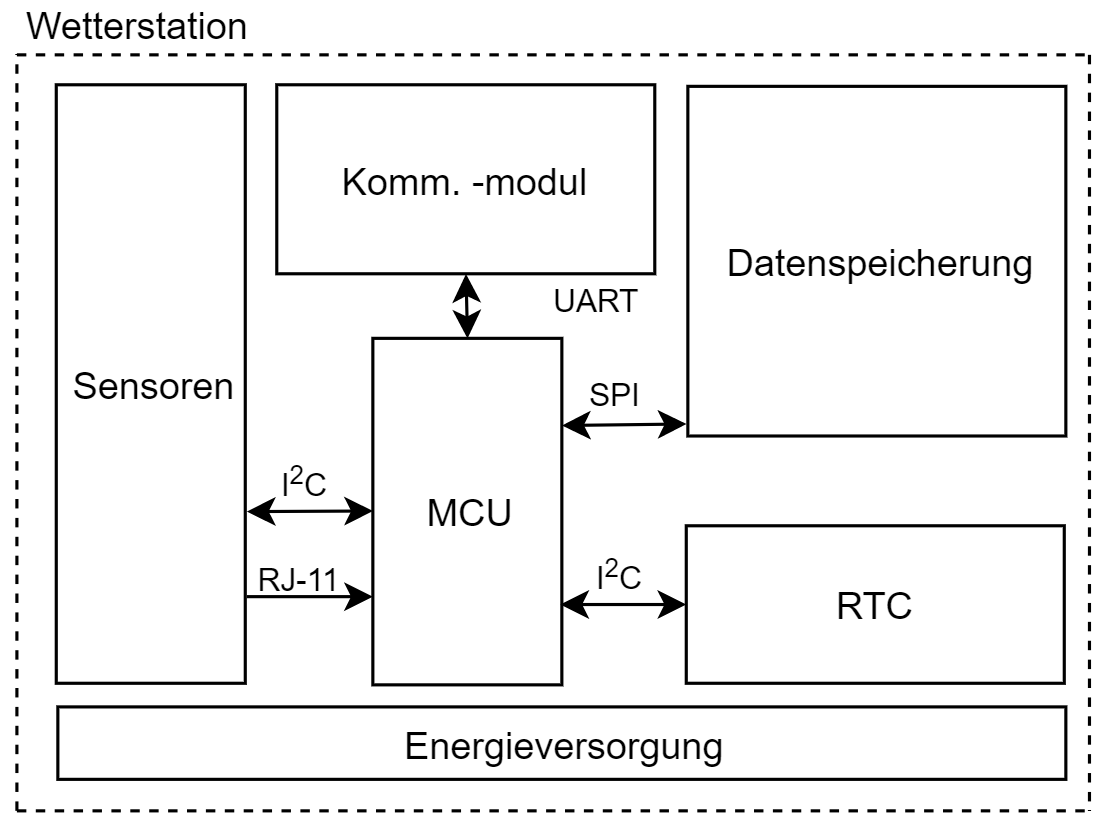
\includegraphics[width=0.9\textwidth]{graphics/Konzeptdiagramme/Grundkonzept.PNG}	
	\caption{Grundkonzept}
	\label{fig:grundkonzept}
\end{figure}

\paragraph{Übersicht:}
Als Zentralrecheneinheit wird eine \textit{Micro-Controller-Unit (MCU)} verwendet. Dieser ist dafür verantwortlich, dass die Daten richtig verarbeitet und an das dementsprechende Modul weitergeleitet werden. Die Messdaten werden in digitaler Form vom Modul \textit{Sensoren} an die \textit{MCU} übertragen. Dieser fügt mit dem \textit{Real-Time-Clock (RTC)} einen Timestamp hinzu, wobei anschließend die Daten in der \textit{Datenspeicherung} nichtflüchtig gespeichert werden. Über das \textit{Kommunikationsmodul} können dann die Daten von Nutznießern abgefragt werden.\\

Das Gesamtkonzept ist, wie in der Abbildung \ref{fig:grundkonzept} grafisch dargestellt, modular aufgebaut. Auf die in diesem Projekt relevanten einzelnen Module wird folgend spezifischer eingegangen.\\

In einem früheren Projekt wurde bereits die Sensorik zur Ermittlung der Lufttemperatur, Luftfeuchtigkeit, Luftdruck, Windgeschwindigkeit, Windrichtung und Regenmenge online erworben und implementiert. Im Projekt 6 wird die Sensorik zur Ermittlung der Sonnenstunden implementiert, sowie die gesamte Sensorik verifiziert und gegebenenfalls optimiert. Nachfolgend wird die Art und Weise erläutert, wie die Messdaten ermittelt werden.\\

\subsubsection{Kommunikationsmodul}
\begin{figure}[h]
\centering
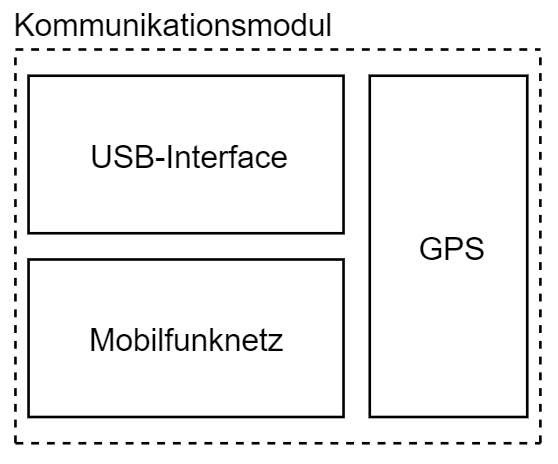
\includegraphics[scale=0.7]{graphics/Konzeptdiagramme/Kommunikationsmodul.PNG}
\caption{Kommunikationsmodul}
\label{fig:kommunikationsmodul}
\end{figure}
Abbildung \ref{fig:kommunikationsmodul} zeigt die verschiedenen Schnittstellen, über welche Daten mit der Umgebung (User) und \textit{MCU} ausgetauscht werden können. Im Rahmen des Projekts 5 wurde das USB-Interface umgesetzt. Mobilfunknetz und GPS sind Teil des Projekts 6.\\

\subparagraph{USB-Interface:}
Über dieses Interface kann mit dem System kommuniziert und interagiert werden. Ein serielles Terminal-Emulationsprogramm (wie z.B. PuTTY) wird dazu benötigt.\\

\subparagraph{Mobilfunknetz:}
Die Einbindung der Wetterstation wird über diesen Block implementiert. Dazu wird ein GSM-Modul benötigt.\\

\subparagraph{GPS:}
Dieser Block sorgt für die Standortbestimmung. Dafür wird ein GPS-Modul auf dem PCB integriert.\\
\subsubsection{Energieversorgung}
\begin{figure}[h]
\centering
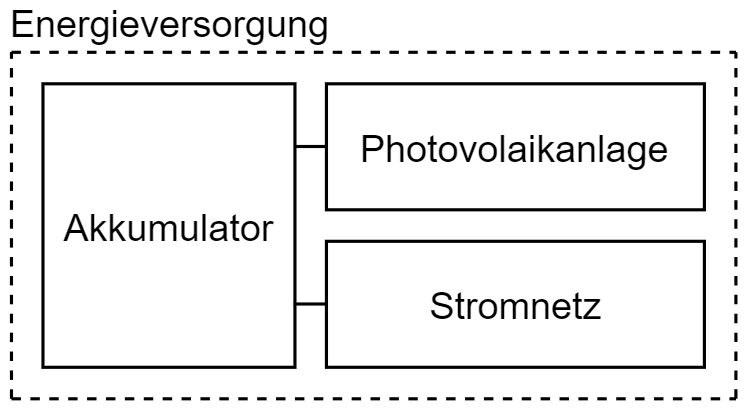
\includegraphics[scale=0.6]{graphics/Konzeptdiagramme/Energieversorgung.PNG}
\caption{Energieversorgung}
\label{fig:Energieversorgung}
\end{figure}

Für die Speisung wird ein Akku verwendet. Gemäss Abbildung \ref{fig:Energieversorgung} soll dieser durch eine Photovoltaikanlage geladen werden. Als Wunschziel soll der Akku austauschbar sein.\\